% !TEX TS-program = pdflatex
% !TEX encoding = UTF-8 Unicode

% This is a simple template for a LaTeX document using the "article" class.
% See "book", "report", "letter" for other types of document.

\documentclass[11pt]{article} % use larger type; default would be 10pt

\usepackage[utf8]{inputenc} % set input encoding (not needed with XeLaTeX)

%%% Examples of Article customizations
% These packages are optional, depending whether you want the features they provide.
% See the LaTeX Companion or other references for full information.

%%% PAGE DIMENSIONS
\usepackage{geometry} % to change the page dimensions
\geometry{a4paper} % or letterpaper (US) or a5paper or....
% \geometry{margin=2in} % for example, change the margins to 2 inches all round
% \geometry{landscape} % set up the page for landscape
%   read geometry.pdf for detailed page layout information

\usepackage{graphbox}
% \usepackage{graphicxbox}
\graphicspath{{img/}}
\usepackage{tabularx}
\usepackage{listings}
\usepackage{amsmath}

% \usepackage[parfill]{parskip} % Activate to begin paragraphs with an empty line rather than an indent

%%% PACKAGES
\usepackage{booktabs} % for much better looking tables
\usepackage{array} % for better arrays (eg matrices) in maths
\usepackage{paralist} % very flexible & customisable lists (eg. enumerate/itemize, etc.)
\usepackage{verbatim} % adds environment for commenting out blocks of text & for better verbatim
\usepackage{subfig} % make it possible to include more than one captioned figure/table in a single float
% These packages are all incorporated in the memoir class to one degree or another...

%%% HEADERS & FOOTERS
\usepackage{fancyhdr} % This should be set AFTER setting up the page geometry
\pagestyle{fancy} % options: empty , plain , fancy
\renewcommand{\headrulewidth}{0pt} % customise the layout...
\lhead{}\chead{}\rhead{}
\lfoot{}\cfoot{\thepage}\rfoot{}

%%% SECTION TITLE APPEARANCE
\usepackage{sectsty}
\allsectionsfont{\sffamily\mdseries\upshape} % (See the fntguide.pdf for font help)
% (This matches ConTeXt defaults)

%%% ToC (table of contents) APPEARANCE
\usepackage[nottoc,notlof,notlot]{tocbibind} % Put the bibliography in the ToC
\usepackage[titles,subfigure]{tocloft} % Alter the style of the Table of Contents
\renewcommand{\cftsecfont}{\rmfamily\mdseries\upshape}
\renewcommand{\cftsecpagefont}{\rmfamily\mdseries\upshape} % No bold!

%%% END Article customizations

\newcommand{\imgtex}{\begin{tabularx}{\textwidth}{@{}c@{ }X@{}}}

%%% The "real" document content comes below...

\title{Inductive Automation Manual}
\author{by CD4017BE}
\date{mod version: 3.7.1}

\begin{document}
 \maketitle
 \tableofcontents
 
 \section{About this manual}  
  Ingame there already is basic information about the blocks and items available in their tooltips if you press SHIFT. So this manual contains the more detailed information about how things work in Inductive Automation. But crafting recipes are not available here, use the Not Enough Items mod to view them ingame. This mod contains its own NEI plug-in so recipes that are crafted using the various machines of this mod are also available. There are some things that can be changed via the config file, so all database values listed here refer to the default config settings. As the ingame tooltips refer to the client config settings they may show wrong values when playing on a server with different settings.

Most screenshots used here are edited to make them fit better into the document and they also could show textures of an earlier mod version, so don't worry if your ingame should look a bit different. 

The information provided here refers to the mod version displayed above.

\newpage
\section{Item \& fluid transport}
\subsection{Machine configuration}
A simple way to transport items or fluids from one machine to another is by placing them next to each other and configure the intended transport using the tabs on the left of their GUIs:\\
\includegraphics[width = \textwidth]{machineCfg}
The tab with the energy pulse icon in upper left is for power connections, the one with the chest icon is for item transport and the one with the tank icon for fluid transport. Each line of the matrix represents one side of the block: B = bottom [-Y], T = top [+Y], N = north [-Z], S = south [+Z], W = west [-X], E = east [+X]. And Each column of the matrix represents the tank or inventory slots that are marked in the same color. By clicking on an element of the matrix you   can change its mode: \\

\includegraphics[]{cfgIn} only input allowed. Input inventories/tanks will automatically drain things out of the neighboring block. \\

\includegraphics[]{cfgOut} only output allowed. Output inventories/tanks will automatically fill things into the neighboring block. \\

\includegraphics[]{cfgBi} input and output allowed. But things won't be transported automatically. \\

\includegraphics[]{cfgNo} inventory/tank/energy can't be accessed at all from this side.\\
Input inventories/tanks are marked by a "I" on top of their column and output inventories/tanks are marked by a "O". Neutral inventories/tanks won't transport things on their own and are marked by a "N", the energy connection is always marked with "E".

There are another two lines on the fluid configuration tab. The one with the lock icon can be used to lock the fluid type of a tank. This way the tank will keep its fluid type when emptied, so no other fluid type can be filled in anymore. Click on an entry to enable/disable this function. The other line with the red crosses will delete the fluid contained in a tank when clicking on its entry.

\subsection{Extraction, injection \& transport pipes}
For greater distances between machines there are three different pipes for each items and fluids available.\\
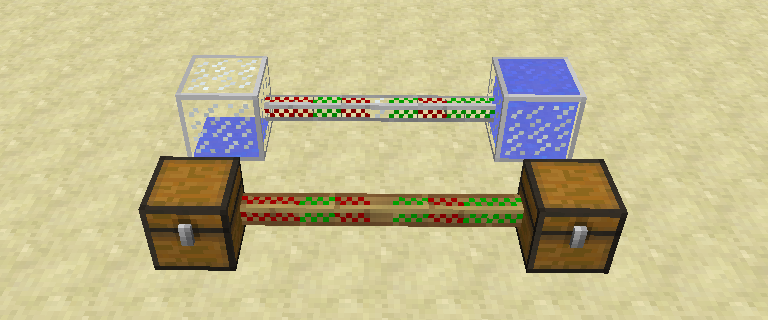
\includegraphics[width = \textwidth]{pipes}
Each item pipe has an internal storage of one stack and is able to transport up to one stack per tick (50ms). By default they will connect to other item pipes and to blocks that have an inventory. Each fluid pipe has an internal storage of 1000L (= 1 Bucket) and is also able to transport 1000L per tick. And these will by default connect to other fluid pipes and to blocks that can store fluids. Connections between pipes or from pipe to block can be disabled by sneak-right-clicking the pipe with an empty hand on the side. Sneak-right-click the side again to reconnect. Connections are marked in different colors depending on their state: A red connection indicates that the pipe will receive things from this side, a green connection indicates that the pipe will output things to this side and no color indicates that no transport will happen on this side. All pipes will try to move their content to other pipes through their output connections. If a fluid pipe has multiple output connections, the contained fluid is evenly distributed. Whereas item pipes try to output in the order B,T,N,S,W,E. Extraction pipes try to extract things from their connected blocks into their internal storage and injection pipes will first try to output the content of their internal storage to connected blocks before they output to other pipes. They also operate in the order B,T,N,S,W,E. \\
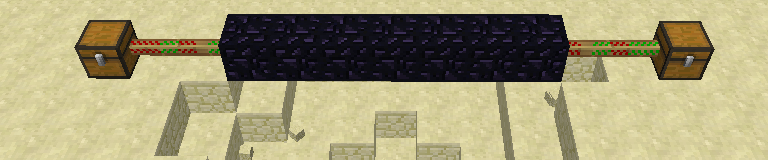
\includegraphics[width = \textwidth]{pipeCovered}
For aesthetics you can right-click any pipe (also energy wires) with a solid block in hand to make the pipe look like this block. The pipe will then also get the hardness and explosion resistance of the covering block. To remove the cover either break the pipe or sneak-right-click it with an empty hand.

\subsection{Fluid \& item pipe filter}
For better control over extraction and injection pipes there are fluid and item pipe filters available. Right-click them on a pipe to insert and right-click on the pipe again with empty hand to remove them. You can only apply one filter to a pipe and that one will be used for all its connections to Blocks. These filters will show their GUI when right clicking their item in the air: \\

\includegraphics[width = 0.5\textwidth]{itemFilter} 
\includegraphics[width = 0.5\textwidth]{fluidFilter}
The 
\includegraphics[align = c]{sendFurtherY} setting lets injection pipes send their contents further to connected pipes if they weren't able insert it into connected blocks. Whereas the 
\includegraphics[align = c]{sendFurtherN} setting lets injection pipes only send things further that are not allowed by the filter, everything else is kept in the pipe until it can be inserted into connected blocks. On extraction pipes this setting has no effect. \\

\includegraphics[align = c]{redstoneOn} lets pipes only extract/insert things if they get a redstone signal and 
\includegraphics[align = c]{redstoneOff} only if they get no signal, otherwise they will always operate. \\
The 
\includegraphics[align = c]{allowFilterY} setting lets pipes only extract/insert the items/fluids listed in the slots, otherwise with 
\includegraphics[align = c]{allowFilterN} only everything else but the listed things are allowed. \\
To configure a fluid type in the fluid pipe filter just put any fluid container containing this fluid into the slots. The number on the right in the fluid filter GUI lets fluid extraction pipes leave at least that amount of liters over in the connected tank when extracting and injection pipes will only fill connected tanks up to this amount if it's greater than 0. Clicking on the light gray +/- will change the number by 1 (left-click) / 100 (right-click) and the dark gray by 10 (left-click) / 1000 (right-click). \\
On item pipe filters use the 
\includegraphics[align = c]{itemLimitY} setting to let extraction pipes leave the listed items with their stack sizes over in the connected inventory or to let injection pipes put these items only up to their stack sizes into connected inventories. In combination with 
\includegraphics[align = c]{allowFilterN} non listed items will be extracted/inserted without limit.
Also the item filter offers some settings for how the filter should compare items with the listed ones: With 
\includegraphics[align = c]{useDamageY} it will look at the damage value of items, with 
\includegraphics[align = c]{useNBTY} it will look at NBT-data of items and with 
\includegraphics[align = c]{useOreDict} it will tread items as the same if they are registered with the same name in ore-dictionary (so for example all copper ingots from different mods are treaded as the same item).

\subsection{Warp pipes}
Unlike normal item or liquid transport pipes, item/liquid warp pipes have no internal buffer and move things instantly. This makes it possible to tranport many different item or fluid types on the same line without having them blocking each other:\\
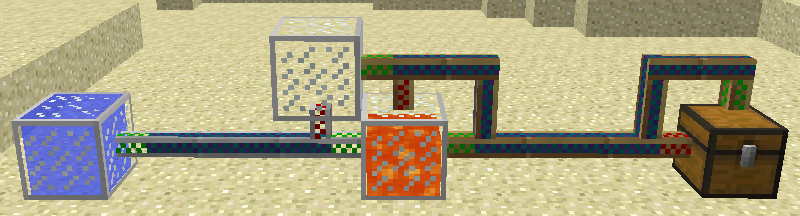
\includegraphics[width = \textwidth]{warpPipes}\\
 Another advancement of warp pipes is that you can have multiple inputs and outputs on the same pipe block with each having its own pipe filter. Right-click an item warp pipe with an item extraction/injection pipe on a side to let it extract/inject items from/to the inventory on that side. Right-click that side again with an item pipe filter to apply it. The same also counts for liquid warp pipes. The transfer rate for item warp pipes is 1 stack/tick for every extracting connection and for liquid warp pipes its 1 fluid type of unlimited amount for every extracting connection. There is a priority setting on \bf item pipe filters \rm to set the the priority of warp pipe destinations. Destinations with higher priority are served first and unfiltered destinations have a priority of 0.

\subsection{Special item \& fluid managing machines}
\imgtex \hline

\includegraphics[align = t]{blockTrash} & \bf Trash: \rm Deletes items and fluids. The right slot of its GUI deletes items and the left slot empties fluid containers. Click on the arrows to enable/disable item/fluid deletion. \\ \hline

\includegraphics[align = t]{blockSorter} & \bf Item Sorter: \rm Routes inserted items into its 5 different internal slots using the 4 item pipe filters that have to be put into the slots right next to them. The cyan slot will take all the items that couldn't go else. All filter functions except amount limit and redstone control are supported. \bf Item transport pipes \rm can be connected directly to this block (without extract/inject) if all transport configurations of a side are set to the same (in/out only).\\ \hline

\includegraphics[align = t]{blockRegulator} & \bf Item Flow Regulator: \rm Has 18 slots of item buffer (red) and moves the contained items into its green and blue slot by splitting their amount at the selected ratio (set both to 0 to disable) and additionally moves items to its green slot if a specified amount of slots is filled (overflow). With 
\includegraphics[align = c]{bigStackFirst} always the item with highest stack size is taken. \\ \hline

\includegraphics[align = t]{blockInterdim} & \bf Interdimensional Wormhole: \rm Teleports entities and players to its linked destination on contact and also item, fluid and energy access from a side to this block is redirected to the neighbor block on the opposite side of its linked destination. By placing this block you get the second block that is linked to it spawned in your inventory. \\ \hline
\end{tabularx}

\subsection{Item and fluid storage}
\imgtex \hline
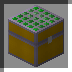
\includegraphics[align = t]{blockMassstorage} & The \bf Mass storage chest \rm has 64 slots (green) with a maximum stack size of 4096 each, this even counts for items which have a usual maximum stack size below 64. Items put into the red slot are automatically sorted into the chest. It's recommended to only use this slot for input because otherwise the stacking doesn't work correctly. Left-click on a slot takes 64 items, right-click 1 item, shift-left-click puts 64 items into your inventory and shift-right-click will fill it with that item as much as possible. When broken the contents are stored in the dropped item.\\ \hline
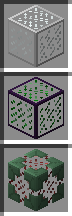
\includegraphics[align = t]{blockTanks} & Basic \bf tanks \rm have a capacity of 64 buckets, \bf mass storage tanks \rm a capacity of 4096 buckets and \bf quantum tanks \rm a capacity of 2097152 buckets. All have two slots in their GUI: the red will empty fluid containers into the tank and the green will fill them. As there is only one slot for each operation, stacked fluid containers are filled/emptied all at the same time. They will keep their content stored in the dropped item when broken. They will also function as fluid containers in their item form. \\ \hline
\end{tabularx} \\\\
\imgtex

\includegraphics[align = t]{blockMatterOrb} & \bf Matter orbs \rm can store 256 different items with a maximum stack size of $2^{31}-1$ each. When placed in the world as block items can only be piped in. A \bf matter interface \rm can be used to view the contents of a matter orb, insert items through the red slot and extract the currently selected item type through the green slot. When configured a redstone signal can be also used to cycle the output to the next type. The matter orb item is usually put into the right slot, the left slot can be used to directly transport items into another matter orb item using the button below.\\ \hline 
\includegraphics[align = t]{blockFluidconverter} & The \bf fluid stabilizer \rm converts 1000L of any fluid into an stabilized fluid item which then can be used as filled fluid container in a tank or to be placed into the world. This conversion requires 1L[= 1 ng] antimatter per 1000L fluid. The machine has three tanks to convert three different fluids simultaneously. \\ \hline
\end{tabularx}

\section{Detector and redstone control}
Some machines in this mod can be controlled by redstone signals (mostly turning them on and off) but for advanced automated systems manually switched levers may be inconvenient so there is a universal sensor block called \bf detector\rm . It's able to check inventory, fluids and energy of its connected block (side marked with 4 green squares on texture). \\
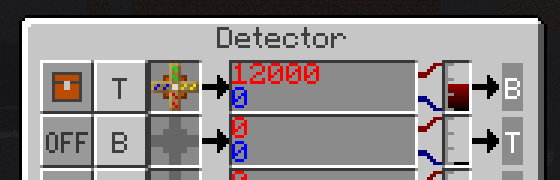
\includegraphics[width = \textwidth]{detector} \\
In its GUI you can set 6 detecting conditions (one for each redstone output side of the block). The first button (most left) sets what should be checked: 
\includegraphics{detectItem} will check the amount of items in the block's inventory, 
\includegraphics{detectFluid} will check the amount of fluid in the block's internal tanks (counted in L or mB) and 
\includegraphics{detectEnergy} will check the amount of energy stored inside the connected block (counted in units of kJ) this also includes the redstone flux energy from Thermal Expansion (1kJ = 10RF) and when attached to cables it will count their internal stored energy (see energy section). The next button defines from which side the connected block should be accessed and the slot can be used to filter the item or fluid detection: put an item here to let the detector only count that item type or a fluid container to only count the fluid type it contains. The button with the $<$ or $>$ sign sets whether the output signal should be on if the detected value is less than the reference value ($<$) or if it needs to be greater or equal to it ($>$). In the text field you can set any number between -2147483648 (negative values usually doesn't make sense but it's possible) and +2147483647 as reference value. If the condition is fulfilled the arrow on the right will turn red and the detector will output a redstone signal to that side.

With Computercraft installed the detector block can be also used as peripheral by computers to directly read inventory, fluid and energy data out of the connected block:
\begin{lstlisting}
0: m = peripheral.wrap("Automation-Detector_0")
1: U, Umax = m.getVoltage(side) --In units of V
2: E, Emax = m.getEnergy(side) --In units of kJ
3: inv = m.getInventory(side)
4: itemID = inv[slot].id
5: damage = inv[slot].dmg
6: stacksize = inv[slot].am
7: tanks = m.getFluidTank(side)
8: fluidID = tanks[i].id
9: amount = tanks[i].am
10: capacity = tanks[i].cap
\end{lstlisting}
1: returns current cable voltage and maximum voltage (both 0 if not connected to a valid cable). 2: returns currently stored energy and energy storage capacity (both 0 if not connected to a valid block). 3: returns a table containing the inventory from the given side of the connected block (or nil if block has no inventory) 4:, 5: and 6: show how to access the item id, damage value and stack size of each contained item with 'slot' as the slot id where the item is stored. 7: returns a table containing all fluid tanks from the given side of the connected block (or nil if block doesn't provide fluid storage) 8: , 9: and 10: show how to access fluid id, stored amount and tank capacity for each tank with 'i' as the tank number. 'fluidID' and 'amount' will be 0 for empty tanks. The 'side' parameter is a number that defines the side from which the connected block should be accessed: 0 = bottom, 1 = top, 2 = north, 3 = south, 4 = west, 5 = east.\\

As complicated circuits or wiring get very big when using minecraft's default redstone components it may be good to have a mod installed that offers compact redstone circuitry (like the Automated Redstone mod I also created).

\section{Energy}
\subsection{Heat \& Steam}
The most basic form of energy is heat. Here it is counted in K (Kelvin), 1K is the amout of heat produced per tick in a normal Furnace (coal has a fuel value of 1600 K, a bucket of lava 20000 K,...). The next type of energy source is steam, its a fluid (gas) so like other fluids its counted in L(liters) or mB (milli buckets) [$1000L = 1m^3 = 1Bucket = 1000mB$] and it should be compatible with steam provided by other mods. Inductive Automation offers two machines to produce it: \bf steam boiler \rm \& \bf lava cooler \rm \\
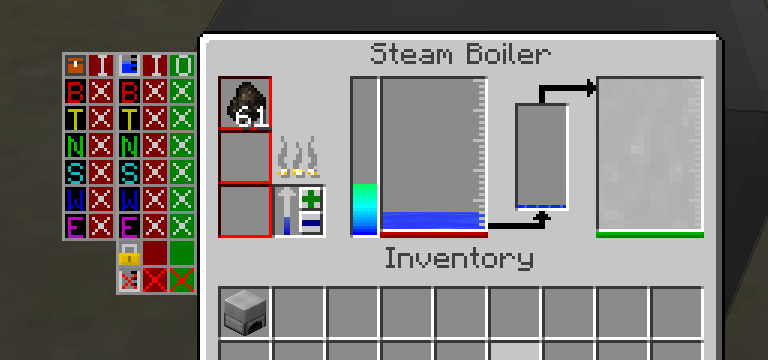
\includegraphics[width = \textwidth]{steamBoiler}
The steam boiler will heat up burning the fuel items in its red slots. This process already produces little 1L steam per K burned (combustion gases). Use the +/- buttons to adjust the burn speed (1-8 K/t). It will stop burning new items when it receives a redstone signal or its heat value reaches maximum. Using heat and the water in its red tank it will additionally produce 250L steam out of 2L water and 50K heat per operation. The operating speed increases with heat level. \\
Reaction formula: $0.04L_{water} + 1K_{heat} \Longrightarrow 6L_{steam}$ at max $8K/t$ \\
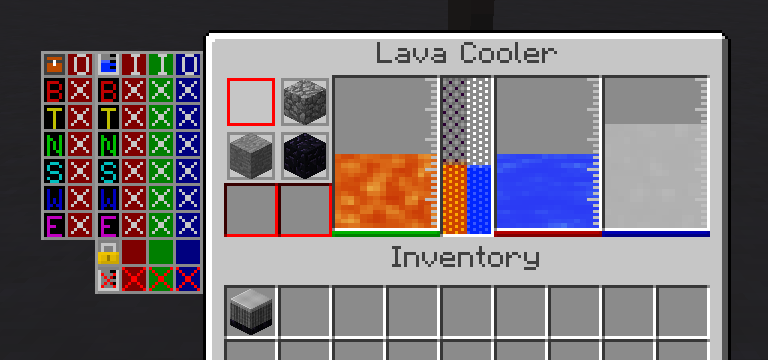
\includegraphics[width = \textwidth]{lavaCooler}
The lava cooler requires water and lava to operate and will always produce 20L steam per tick while operating. Apply a redstone signal to let it stop running. It has different operating modes that produce different items as by product. These are put into the red slots, if they are full the machine will stop running. To select a mode, just click on its slot, it should then get a red frame around it. These modes require different amounts of lava, water and time which is shown in the following table:\\
\begin{tabular}{| l | c | c | c | c | c |}
\hline
\bf By product & \bf Lava & \bf Water & \bf Ticks & \bf Steam & \bf Energy/lava \\
\hline
Nothing & 10L & 10L & 50[2.5s] & 1000L & 20kJ/L \\
Cobblestone & 4L & 4L & 20[1s] & 400L & 20kJ/L \\
Stone & 40L & 80L & 200[10s] & 4000L & 20kJ/L \\
Obsidian & 1000L & 500L & 2500[2m5s] & 50000L & 10kJ/L \\
\hline
\end{tabular} \\
Currently the steam pneumatic compressor is the only operating machine that is directly powered by steam, most other machines require electricity.

\subsection{Electric generators}
Electric energy (E) which is used by most machines is counted in J (Joules) or kJ (kilo Joules) [1kJ = 1000J] and energy generation, transfer or consumption per tick (P) is counted in W (Watts) or kW (kilo Watts) [1000W = 1kW = 1kJ/t = 1000J/t]. It can be produced using these machines:\\
\imgtex \hline

\includegraphics[align = t]{steamEnergy} & \bf Steam engine, steam generator \rm and \bf steam turbine \rm generate electric energy by converting steam back into water: $1L_{steam} \Longrightarrow  0.005L_{water} + 200J$ Their operating speed depends on the fill state of their steam tank, it's at maximum when 50\% filled. Their maximum power is shown in this table: \begin{tabular}{| l | c | c | c |} \hline
\bf Machine & \bf Max power & \bf Max steam in & \bf Max voltage \\ \hline
Steam engine & 4kW & 20L/t & 240V \\
Steam generator & 24kW & 120L/t & 1200V \\
Steam turbine & 120kW & 600L/t & 1200V \\ \hline
\end{tabular} \\ \hline

\includegraphics[align = t]{solarPanels} & \bf Solar panels \rm generate electric energy from light. Their power multiplier is: $(Skylight^3 + Blocklight) / 3375$ , where the light values can be 0-15. As they do also produce energy from block light like torches skylight is 225 times more efficient. This table shows the energy output of the two solar panel tiers under various conditions:
\begin{tabular}{| l | c | c | c | c | c |} \hline
\bf Solar panel & \bf Day & \bf Night & \bf Rain & \bf Block & \bf Max voltage\\ \hline
Basic & 500W & 9.48W & 256W & 2.22W & 240V\\
High power & 4053W & 129W & 2101W & 53.3W &  1200V\\ \hline
\end{tabular}\\ \hline

\includegraphics[align = t]{hydrogenFuelCell} & The \bf hydrogen fuel cell \rm generates electric energy and steam out of hydrogen and oxygen gas: $2L_{hydrogen} + 1L_{oxygen} \Longrightarrow 1L_{steam} + 1.8kJ$. The operating speed depends on the fill state of its internal energy buffer (16MJ) which functions like an energy storage unit. Its at maximum producing 144kW when empty and turns off when more than 50\% filled. Max voltage: 8000V. \\ \hline
\end{tabularx}

\subsection{Energy transport \& storage}
Electric energy is transported through cables where every machine that operates with electricity already acts like a cable there are additionally three types of cables to connect distant blocks. Relevant variables for electric energy transport  here are U(Voltage) counted in V(Volt), I(Current) counted in A(Ampere), R(Resistance) counted in Ohm,  and the already mentioned E[J](energy) and P[W](power) as well as T(time) in t(game ticks: 1t = 0.05s if not lagging).

A machine that is producing energy will fill it into its internal cable. Cables can already store a small amount of energy as they function like small electric capacitors, their stored energy is calculated by: $E = U^2 * n$ , where n is the amount of connected cable blocks, so for example a single cable storing 40kJ has a voltage of 200V. When energy is added to the cable its voltage will increase until it reaches its maximum voltage (shown as 'Umax' in their tooltips), then anymore added energy is wasted. The voltage of a cable can be seen by linking a \bf volt meter \rm to them.

Machines that consume energy have a working resistance (shown as 'Rwork' in their tooltips or configurable in their GUI, otherwise 1 Ohm) and a reference voltage that usually is 0V. The energy they can receive from their cable is calculated by: ${P = \frac{U_{wire}^2 - U_{ref}^2}{R_{work}}}$ , so a machine with a working resistance of 25 Ohm that is supplied with 750V would run at 22.5kW. This way it is also possible to calculate their operating speed: ${T^{-1} = \frac{P_{supply}}{E_{use/op}}}$. Energy is only taken from a cable if the machine requires it. 
\imgtex

\includegraphics[align = t]{RworkCfg} & In some machines their working resistance can be configured using this part of the GUI. The bar right next to the number displays the power the machine would receive with this setting. Note that while a low resistance means fast operation it may also cause other connected machines to receive less energy or at 1 Ohm even no energy at all while this machine is running. That's because the voltage of a cable drops when energy is taken from it. \\
\end{tabularx}

As machines usually have no internal energy buffer (except the energy collected for their current operation) and the amount of energy that a cable can hold is very limited, it is recommended to use energy storage units as soon as possible. These will try to hold the voltage of their connected cables at their reference voltage (configurable in their GUI) by transferring energy into their internal buffer from the cables or vice versa (this transfer is shown above the storage bar in their GUI). With multiple storage units connected to one network those with higher reference voltage will drain first and those with low voltage will fill first. The amount of power emitted or received can be also calculated with the power supply formula above using a resistance of 1 Ohm (negative values indicate emitting power). Example: An ESU set to 800V would transfer ${800^2 - 200^2 = 600kW}$ to an ESU set to 200V.

There is a small loss on basic cables when transferring power, which depends on the cables' conductive resistance (show as 'Rcond' in their tooltips) and the current at which the power is conducted ($I_{cond}$): ${P_{loss} = I_{cond}^2 * n * R_{cond}}$ , where n is the amount of cables and ${I_{cond} = \frac{\Delta U}{R}}$. So to reduce power loss you could transfer power at higher voltages and higher working resistance or use cables with lesser conductive resistance (Super conductive hydrogen wire has no loss at all) or build a smaller network if possible. Usually the power loss is very small and this way negligible.

These tables list the different types of wires and energy storage units: \\
\begin{tabular}{| l | c | c | c |} \hline
\bf ESU-type & \bf Capacity & \bf Max voltage & \bf Max I/O power \\ \hline
Single-cell & 16MJ & 240V & 57600W \\
Octa-cell & 128MJ & 1200V & 1440kW \\
Crystal-cell & 1024MJ & 8kV & 64MW \\ \hline
\bf Wire-type & \bf Resistance & \bf Max voltage & \bf Max power \\ \hline
Copper & 0.01Ohm & 240V & 57600W \\
Conductive & 0.001Ohm & 1200V & 1440kW \\
Hydrogen & superconductor & 8kV & 64MW \\ \hline
\end{tabular}\\

\bf Final note: Don't connect energy cables or machines in a circle! Because of negative interferences the energy won't be transported properly through the whole network anymore. \rm You can disconnect machines using their energy connection tab and cables by sneak-right-clicking them.

\subsection{Voltage Transformer}
Sometimes it may be necessary to connect the energy of different machines or cable networks at different voltages with each other. In this case a voltage transformer or energy link is needed: \\
\imgtex \hline

\includegraphics[align = t]{blockTransformer} & \bf Voltage transformers \rm have two opposite sides that connect to cables which are indicated by 'HV' and 'LV' on texture. They will exchange energy between the connected cables so that ${U_{HV} = x * U_{LV}}$ , where x is the voltage factor that can be set in their GUI. As they have no internal cable themselves, they are not limited to a maximum voltage.\\ \hline

\includegraphics[align = t]{blockELink} & \bf Energy links \rm have one side (marked with blue square dot) where you can place any block that can store energy [Cables(see above section), ESUs, RF devices]. They will function similar to ESUs but use the connected block as energy buffer and you can set two different reference voltages rather than just one: 'Umax' for full Storage and 'Umin' for empty Storage, the actual Uref results as a linear interpolation between them depending on the fill state. There are two types of energy link that differ in their maximum voltage: the basic has 1200V and the HV has 8000V.  As energy links also connect to Thermal Expansion RF storing blocks/conduits they can be used as bidirectional energy converter with a ratio of: ${1RF = 100J}$. \\ \hline
\end{tabularx}
All these machines can be configured in their GUI to be controlled by redstone. Turning them off means they won't transfer energy.

\subsection{Tesla transmitters}
\bf Tesla transmitters \rm offer a wireless and lossless (in reality this would be very lossy but its minecraft) energy transport over long distances. They have an internal cable that only connects on their bottom side and has a very high maximum voltage (see table below) so it's recommended to connect them to your energy network using voltage transformers or energy links. They will exchange energy with all other Tesla transmitters in the world that are set to the same frequency (can be set in their GUI). This energy transfer is calculated like so: ${P_{A to B} = \frac{U_A^2 - U_B^2}{d^2}}$ , where d is the distance between them in meters(blocks). So higher voltage differences increases energy transport and higher distances decrease energy transport. Inserting an Ender Matrix item into Tesla transmitters (by right-click) will reduce the calculated distance to be never more than 200m even across dimensions (needs to be installed on both connected transmitters). This table shows some technical data about the two  available Tesla transmitter types:\\

\includegraphics[align = m]{blockTesla}
\begin{tabular}{| l | c | c | c |} \hline
\bf Type & \bf Max voltage & \bf Capacity & \bf $P_{max @ d=200m}$ \\ \hline
LV & 24kV & 576MJ & 14.4kW \\
HV & 120kV & 14.4GJ & 360kW \\ \hline
\end{tabular} \\

\subsection{Antimatter}
Antimatter is used for some end game machines and tools and is counted in ng(nano gram), ug(micro gram) or mg(milli gram)[1g = 1.000mg = 1.000.000ug = 1.000.000.000ng]. It can be transported as regular fluid with 1L = 1ng. \\
\imgtex
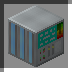
\includegraphics[align = t]{blockAMFabricator} & It is produced by the \bf antimatter fabricator \rm out of energy at a ratio of $160ng = 14400kJ$. It can do up to one operation (160ng) per tick and will turn 0.2L liquid helium into 160L gaseous helium for cooling. It operates with $R_{work}$ = 1 Ohm and has a configurable reference voltage.\\

\includegraphics[align = t]{blockAntimatterTank} & The \bf antimatter tank \rm is a fluid tank that only allows antimatter and it has a capacity of 160000000L (160mg). Antimatter can be also stored in other fluid tanks but this one has a much bigger capacity and when filling fluid containers its fill rate will increase linearly over time allowing fast and precise filling (useful to fill an antimatter bomb). \\
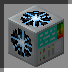
\includegraphics[align = t]{blockAMAnnihilator} & Antimatter can be turned back into energy (at the same ratio it was produced) using the \bf antimatter annihilator\rm, which also requires liquid helium as coolant ($\frac{1}{800}L_{liquid} \rightarrow 1L_{gas}$ per 1ng). The operating speed depends on the fill state of its internal energy buffer (128MJ) which functions like an energy storage unit. Its at maximum producing 14400kW when empty and turns off when more than 50\% filled. Max voltage: 8000V.


\end{tabularx}

\section{World interacting machines}
\imgtex

\includegraphics[align = t]{itemSelectionTool} & Some of these machines operate in a selectable working area. This area needs to be set using the \bf selection tool \rm item. Sneak-right-click on a compatible machine to link it to that machine and sneak click in air to switch between its operating modes: \\
\end{tabularx}
\begin{tabularx}{\textwidth}{@{} l @{ } X @{}}
\bf Set point: & \rm right-click on a block sets the area to contain only that block. \\
\bf Add point: & \rm right-click on a block expands the area to contain that block. \\
\bf Expand: & \rm right-click in air expands the area by one block into the direction looking at. \\
\bf Contract: & \rm right-click in air contracts the area by one block on the side looking at . \\
\bf Move: & \rm right-click in air moves the area by one block into the direction looking at. \\
\bf Configure: & \rm right-click in air to open the configuration GUI of the linked machine or sneak-right-click on a machine to open its configuration GUI without linking it. \\
\end{tabularx}
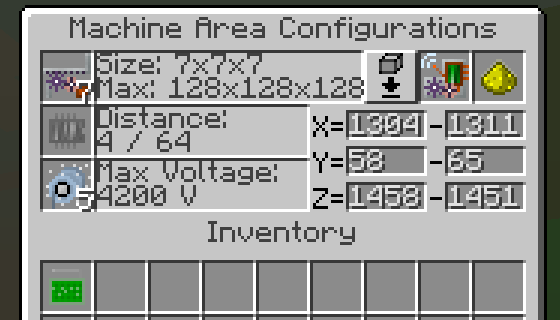
\includegraphics[width = \textwidth]{selectionTool} \\
Put a piece of glowstone dust into the upper-right slot to make the selected area be visible in the world as colored hologram box. The 6 text fields below can be used to set the area by editing its bounding coordinates. The button left next to the area visibility indicator is used to copy the area of one machine to another, to do this just sneak-right click the first machine in any mode except 'configure' to link it and then open the second machine's configuration GUI by sneak-right-clicking it in 'configure' mode and finally click the button to copy the first machine's area to the second machine. The slots on the left are used for upgrades: Every \bf tool motion frame \rm item put into the upper slot increases the machine's maximum area size in all 3 directions and the maximum distance between the machine and the nearest side of its area by 100\% of its original. Every \bf ender matrix \rm item put into the center slot increases the distance by another 400\% of the value that was already increased above (useful to operate from far away). And every \bf superconductor coil \rm item put into the bottom slot increases the machine's maximum cable voltage by 50\% of its original (higher voltages allow greater power supply). These upgrade items are not consumed and can be taken out or will drop when breaking the machine. However removing upgrade items may cause the selected area to be auto corrected to the allowed maximum bounds and distance (working at a place it shouldn't) or cause energy waste by a lowered maximum voltage, so take care.

\subsection{Fluid collector, fluid vent \& magnet}
\imgtex

\includegraphics[align = t]{blockCollector} & The \bf fluid collector \rm will try to remove any fluid block that is directly in front of its oriented face (iron vent texture) and fill it into its internal tank when set to default collection mode. In $O_2$ or $N_2$ mode it requires air in front of it and will produce oxygen gas at 160L/t or nitrogen gas at 100L/t. \\ \hline

\includegraphics[align = t]{blockVent} & The \bf fluid vent \rm will place fluids contained in its internal tank into the world. It will fill all space that is connected to its oriented face and that is below or even to it (above or even for gases). The number in its GUI sets the maximum path length from this block to a placed fluid. It can be set to 127 blocks at maximum. The button next to it defines whether this machine's operation should cause block updates (when filling water better turn it off to prevent automatically generated water source blocks interfering with the filling algorithm). \\ \hline
\includegraphics[align = t]{blockMagnet} & The \bf magnet \rm will pickup dropped items and put them into neighboring inventories and it will also pull entities towards it consuming a very small amount of energy. It operating range depends its cable voltage: $d = \frac{U_{cable}}{64V}m$. It has a maximum voltage of 8000V and consumes 0.1W per entity or item.
\end{tabularx}


\subsection{Pump}
The \bf pump \rm will remove all fluid blocks inside of its cuboid working area and fill them into its internal tank. Like the fluid vent it also has a button to turn block updates on or off and a number selection. This number sets the maximum path length for pumping connected fluid lakes outside of the selected area. It also has a maximum of 127 blocks and setting it to 0 will only drain the selected area. This machine requires energy to pump fluid source blocks. With block updates turned off also non source blocks will be removed at 25\% energy cost. The area will be processed from top to bottom at maximum speed of 1 block/t\\
\imgtex
\includegraphics[align = m]{blockPump} &
\begin{tabular}{| c | c | c | c |} \hline
\bf $U_{max}$ & \bf $R_{work}$ & \bf Energy usage & \bf max area size[xyz] / distance \\ \hline
1200V & 25 Ohm & 8kJ/block & 16 x 64 x 16 / 8 blocks \\ \hline
\end{tabular} \\
\end{tabularx}

\subsection{Automatic mining}
The \bf automatic miner \rm will try to remove all blocks inside of its cuboid working area, placing the dropped items into its internal inventory (green slots). It will stop running when its inventory is full. \bf Drills \rm are required in the red slots to break blocks that can't be harvested by hand. They come in 3 tiers:\\
\begin{tabular}{| l | c | c | c |} \hline  
\bf Type & \bf Harvest level & \bf Durability & \bf Energy cost \\ \hline
Stone & stone tools & 4096 & 66,7\% \\
Iron & iron tools & 8192 & 50\% \\
Diamond & diamond tools & 16384 & 25\% \\ \hline
\end{tabular} \\
Drills can be enchanted in an anvil using enchanted books or tools: \\
\begin{tabular}{| c | c |} \hline
\bf Enchantment & \bf Function \\ \hline
Silktouch & mines with silktouch \& $2x$ energyUse \\ \hline
Fortune & mines with fortune \& $(1+0.6*lvl)x$ energyUse \\ \hline
Efficiency & $(1+0.3*lvl)x$ drill efficiency \\ \hline
Unbreaking & $(1+0.33*lvl)x$ effective durability \\ \hline
\end{tabular} \\
Blocks are always harvested using the lowest available drill tier that is able to break it which will then lose 1 durability per block (no drill is used when harvestable without tools). The energy required is : ${E_{use} = 40kJ * Hardness * EnergyCost}$ , where 'EnergyCost' is the power multiplier of the used drill or 1 if mined without and 'Hardness' is the hardness value of the mined block (stone = 1,5). 

The miner can be (re-)started with a redstone signal of min. strength 8 and will emit a redstone signal of strength 7 when finished or turned off.\\
\imgtex
\includegraphics[align = m]{blockMiner} &
\begin{tabular}{| c | c | c | c |} \hline
\bf $U_{max}$ & \bf $R_{work}$ & \bf max area size[xyz] / distance & \bf max speed \\ \hline
1200V & 25 Ohm & 16 x 64 x 16 / 8 blocks & 16 blocks/t \\ \hline
\end{tabular}
\end{tabularx} \\
With the computer craft mod installed you can wrap a miner as peripheral and control it using these commands:
\begin{lstlisting}
0: m = peripheral.wrap("Automation-Miner_0") --(example name)
1: sX, sY, sZ = m.getAreaSize() 
2: b = m.isBlockAt(x, y, z) 
3: success = m.mineBlock(x, y, z, doEvents)
4: x, y, z, isMined = os.pullEvent("mine_block")
5: m.clearQueue()
6: m.stopMining()
\end{lstlisting}
1: returns the size of the selected area. 2: returns true if there is a mineable block at the given position. 3: adds the mining of the block at given position to the machines processing queue and returns true or returns false if the processing queue is full (contains 16 operations). The miner will try to process these operations during the next game tick. The 'doEvents' parameter is optional and when given with a value of true whenever an operation is done the computer will receive a "mine\_block" event (4:) with the x, y, z position of the mined block and true if it was mined or false if there was no block to mine. 5: will clear the processing queue so all undone operations are canceled. 6: turns the miner off (miner must be off when controlled by computers otherwise 'mineBlock' commands return with an error). All coordinates are relative to the selected operating area and have values of: $x=\{0 \dots sX-1\}$, $y=\{0 \dots sY - 1\}$, $z=\{0 \dots sZ - 1\}$.

\subsection{Automatic building}
The \bf automatic builder \rm can build various even complicated structures out of blocks and fluids inside of its working area. The structure to build is defined in its GUI: \\
\includegraphics[width = \textwidth]{builder} \\
The building is done layer by layer during the different operating steps: 

At first it will build the edges of the cuboid using the materials configured in the upper three slots indicated with "Frame". The vertical aligned edges use the cyan "Y"-slot, the Z-axis aligned use the magenta "Z"-slot and the X-axis aligned use the "X"-slot. 

Next the surfaces (including their adjacent edges and corners if not already build in previous step) of the cuboid are build using the materials configured in the 6 slots indicated with "Walls" (B = bottom face, T = top face, N = north, S = south, W = west and E = east).

And finally the cuboid is filled with stacked layers of the materials in the 8 numbered slots at the bottom. The bottom right button sets the orientation of these layers: "XZ" will orient them in horizontal planes that are vertically stacked upwards, "XY" will orient them in vertical XY-planes that are stacked southwards and "ZY" will orient them in vertical ZY-planes that are stacked eastwards. The material layers are placed in the order of the slots (1-8). The numbers below the slots set the thickness of the individual material layers in blocks (slots with a thickness of 0 are skipped). If the selected area is bigger than the thickness of all configured layers together then they are iterated to fill up the rest.

The builder will leave all layers which have empty slots with air (or the blocks that were there before as the builder can't break any blocks).

Clicking the button on top-left will start or cancel the building process, while working it will show the current operation step otherwise it shows "Inactive". The red slots in the bottom are where the required materials are taken from. If a material isn't available when needed the machine will wait for it. Use fluid container items (like fluid tanks) to let the builder place their contained fluids.

Here is an example configuration and its building: \\
\includegraphics[width = 0.5\textwidth]{buildCfgEx} \includegraphics[width = 0.5\textwidth]{buildingEx} \\
If cuboid rooms with walls and floors out of just one block type look too boring, you could also put \bf building texture \rm items instead of blocks into the configuration slots. They contain a rectangular (2D) area with a maximum size of 32x32 blocks made out of up to 15 different types + air and are created out of paper in the \bf texture drawing table\rm . The GUI of this machine functions similar to a painting program but uses blocks and fluids instead of colors: \\
\includegraphics[width = 0.5\textwidth]{textureDrawing} \includegraphics[width = 0.5\textwidth]{textureBuildEx} \\
The 15 holo-slots on the right form the material palette of the painted texture. Right-click on a slot to set its item and left click will select it (blue frame) without deleting the contained item. Below there are 6 tool modes available (the currently selected has a red frame): \bf Drawing \rm sets the clicked pixels to the current selected material. \bf Filling \rm fills all connected pixels of the material clicked on with the selected material. \bf Replacing \rm will replace all pixels of the clicked material with the selected material. \bf Selecting \rm changes the selected area (green rectangle), left- and right- click to set the two opposite corners of the selection. The 'fill', 'replace', 'clear', 'mirror', 'flip' and 'rotate' operations are only performed inside the selection. \bf Copy \rm will copy the selected area to the position left-clicked on, where the green filled square is the anchor. Right-click sets the anchor position. \bf Moving \rm will move the selected area (functions like copy). The 4 buttons left next to the tool modes will \bf rotate \rm (only works with square selections), \bf clear \rm , \bf mirror \rm or \bf flip \rm the selected area. The other two buttons will save or load the texture from or to the item in the slot below. When a building texture item is created in can be named using the text field. The +/- buttons below are used to change the size of the texture (right-click changes by 8) and the offset position. The offset position defines where the texture will start relative to the operating area when later build. The \bf extension behavior \rm which is set using the button at bottom left defines what should be build outside of the texture if it's smaller than the operating area of the builder. There are 4 different modes: build nothing, continue with the outer edges, iterate the texture or iterate the texture mirrored. \\
When build in layers the texture will be positioned as follows: \\
\begin{tabular}{| c | c | c |} \hline
\bf layer orientation & \bf texture right & \bf texture up \\ \hline
XZ-horizontal & world east & world south \\
XY-vertical[E,W] & world east & world up \\
ZY-vertical[N,S] & world south & world up \\ \hline
\end{tabular} \\

In case you don't just want to build cuboid structures there is another device called \bf 3D-vertex shematic printer \rm :\\
\includegraphics[width = \textwidth]{vertexPrinter} \\
The list on the right contains all polygons of your current structure. To add a polygon, click on \bf NEW\rm, select it and add vertices to it by clicking on \bf ADD\rm . A triangle needs 3 vertices, a quad 4, a pentagon 5, and so on. There are two ways to set the block coordinates of a vertex: You can either select it in the list on the left and enter the X-Y-Z-coordinates using the text fields (numbers are in blocks relative to the operating area's edge with lowest x,y,z coordinates), or you use a \bf vertex selection tool\rm . The U and V coordinates are only important if you want to use building textures and define the position in the texture. Clicking on \bf AUTO TEX \rm will automatically set the texture coordinates equal to the block coordinates.

The builder will build the polygons in form of walls: the +/- number selection defines the texture or material slot to use (stack slots 0-7), the text field next to it defines the thickness of the wall and the small button defines the direction in which the thickness should be applied. This device will render your structure as hologram into the world, where the block itself would be in the corner of the builder's operating are that has lowest x,y,z-coordinates. Every polygon is rendered twice: once for the front and once for the back side of the wall. The color indicates the material/texture slot used and the currently selected polygon is rendered less transparent.

When using the \bf vertex selection tool\rm ,sneak-right-click cycles through the vertices of the currently selected polygon and right-click sets the currently selected vertex to the block click position (clicked on block) or the players feet position (clicked in air) rounded to the next block corner.

There are two ways to save a structure: when saved on a \bf book \rm it will remain exactly the same when loaded again but it can't be put into a builder. Therefore you need to save it on \bf paper \rm which will split every polygon into triangles. When loading a structure from paper, it will still look the same but contains more polygons with only three vertices each instead. To actually build a structure just put the paper its stored on into the stack slot on the right of the builder interface and supply the intended materials or textures. The builder will then build your structure instead of the usual filling operation.\\
\includegraphics[width = \textwidth]{vertexEx}\\

And if you want to do very special things like spheres, waves, or other smooth rounded structures you can  control the builder using computer craft if installed:
\begin{lstlisting}
0: m = peripheral.wrap("Automation-Builder_0") --(example name)
1: sX, sY, sZ = m.getAreaSize() 
2: b = m.isBlockAt(x, y, z) 
3: success = m.setBlock(x, y, z, slot, doEvents)
4: x, y, z, isSet = os.pullEvent("set_block")
5: m.clearQueue()
6: m.stopBuilding()
\end{lstlisting}
1: returns the size of the selected area. 2: returns true if there is a block at the given position that can't be replaced by the builder (tall grass or fluids can). 3: adds the placement of a block at given position to the machines processing queue and returns true or returns false if the processing queue is full (contains 16 operations). The builder will try to process these operations during the next game tick. The 'slot' parameter defines which of the 17 configurations slot to use as material and must have a value of $\{ 0 \dots 16 \}$ (0,1,2 = frame slots; 3,4,5,6,7,8 = walls slots; 9-16 = fill slots). The 'doEvents' parameter is optional and when given with a value of true whenever an operation is done the computer will receive a "set\_block" event (4:) with the x, y, z position of the placed block and true if it was placed or false if there already was a non replacable block before. 5: will clear the processing queue so all undone operations are canceled. 6: will cancel the builder's current building operation that was started via the button in its GUI (manual defined and computer controlled building aren't allowed at the same time). All coordinates are relative to the selected operating area and have values of: $x=\{0 \dots sX-1\}$, $y=\{0 \dots sY - 1\}$, $z=\{0 \dots sZ - 1\}$. \\

Here an example program that would build a simple hollow sphere out of the material put in the Y-edge slot (at max speed of course):
\begin{lstlisting}
m = peripheral.wrap("Automation-Builder_0") --if modem connected
sX, sY, sZ = m.getAreaSize()
if sX ~= sY or sY ~= sZ then return end --Area must be a cube
radOut = sX * 0.5
radIn = radOut - 1 --using a sphere wall thickness of 1 block 
for x = 0, sX - 1 do
 for y = 0, sY - 1 do
  for z = 0, sZ - 1 do
   dX = x + 0.5 - radOut
   dY = y + 0.5 - radOut
   dZ = z + 0.5 - radOut
   sqd = dX * dX + dY * dY + dZ * dZ
   if sqd <= radOut * radOut and sqd > radIn * radIn then
    while not m.setBlock(x, y, z, 0) do sleep(0.05) end
   end
  end
 end
end
\end{lstlisting}
Finally this table shows some technical data about the machine: \\
\begin{tabular}{| c | c | c | c | c |} \hline
\bf $U_{max}$ & \bf $R_{work}$ & \bf Energy usage & \bf max area size[xyz] / distance & \bf max speed \\ \hline
1200V & 25 Ohm & 25kJ/block & 16 x 16 x 16 / 8 blocks & 16 blocks/t \\ \hline
\end{tabular} \\

For special block placement (stairs, pipe covers, etc.) use a configured \bf block placement controller \rm instead of the block item. Right-click it in the air to open its GUI: \\
\includegraphics[width = \textwidth]{placementController} \\
Its configuration will cause a right-click operation for every item put into the 8 slots on top (in the order they appear). The required items will be taken from the inventory of whatever is using the placement controller and then the results (if any) will be put back into it. If the setting on top right is enabled then a temporary block will be placed if there is no other block available to place the items against. The settings on the bottom define how the currently selected item (green frame) should be right-clicked: The setting on the left defines the looking direction. The numbers in the text fields define the position where the bounding box of the block clicked against should be hit (bottom-top: Y=0-1, north-south: Z=0-1, east-west: X=0-1). The sneak-setting defines whether the item should be right-clicked while sneaking or not and the last setting defines whether only the given item is alowed for the operation or if different metadata / damage versions of the item should be also accepted (usefull for tools that take durability).

The block placement controller can be also manually used by right-clicking it on a block. It will then perform the configured placement next to that block, taking the required items from your inventory (mainly used to check if the placement would work like it was intended).

\subsection{Automatic farming}
The \bf automatic farm \rm places and harvests plants in its operating area. These need to be configured in its GUI:\\
\includegraphics[width = \textwidth]{farm} \\
It will try to plant the plantable items configured in the 8 green slots on top into the operating area wherever possible by taking the items from the green inventory below. If it can plant multiple different plants on a block, it will randomly choose one using their configured stack sizes as probability ratio. 

For special planting operations (ex.: bone meal on grass to get tall grass \& flowers) it is possible to use \bf block placement controllers \rm in the planting configuration (explained in previous section). Note that the first slot in the configuration of the block placement controller won't be placed, here it is instead used to configure the required "soil" to plant the following items on.

The harvest configuration is done by inserting a \bf pipe item filter \rm in the red slot on top. The farm will harvest every block that drops at least one item that matches with the filter. But it's only able to break blocks that don't need a tool to be harvested. All filter functions are provided but some have a different functionallity here: The \includegraphics[align = c]{sendFurtherN} setting will additionally use the silk-touch result of blocks and with the \includegraphics[align = c]{itemLimitY} setting the configured item stacksizes are used to restrict the allowed block metadata value ($1 \dots 15 \rightarrow 1 \dots 15$; $16 \rightarrow 0$; $17 \dots 64 \rightarrow any$).

Dropped items are automatically sorted to the green inventory if configured to be planted again and if there is space, otherwise they are put into the red inventory. The machine stops running when its inventory is full.

The machine can process 1 block/t but will skip air blocks much faster. Its energy and operating area data is shown in this table:\\
\begin{tabular}{| c | c | c | c | c |} \hline
\bf $U_{max}$ & \bf $R_{work}$ & \bf Energy usage & \bf max area size[xyz] / distance \\ \hline
1200V & 25 Ohm & 25kJ/block & 12 x 16 x 12 / 8 blocks \\ \hline
\end{tabular}

\subsection{Machine synchronizing}
Using a \bf machine co-op synchronizer \rm it is possible to extend the functionality of a machine by the functionality of  another machine. When connecting two machines in this way, there is always one machine being master and the other one being slave. First link the \bf machine co-op synchronizer \rm to the slave machine by sneak-right-click. Then sneak-right-click the master machine with a selection tool in configure mode to open its upgrade inventory and insert the linked machine co-op synchronizer. It's also possible to link up to three different machines in a chain (ex. Builder with Miner and Miner with Pump). The machine combinations available are shown in this table: \\

\begin{tabular}{| c | c | l |} \hline
\bf Slave \rm & \bf Master \rm & \bf Function \rm \\ \hline
Pump & \begin{tabular}{ c } Miner \\ \hline Builder \end{tabular} & Adds ability to remove fluids.\\ \hline
Miner & \begin{tabular}{ c } Builder \\ \hline Farm \end{tabular} & Adds ability to break blocks.\\ \hline
Builder & \begin{tabular}{ c } Pump \\ \hline Miner \end{tabular} & Fills up the hole afterwards.\\ \hline
\end{tabular}\\

If a builder has a miner or pump as slave machine, it can place new blocks into preexisting blocks/fluids by removing them. Using a \bf remove block pattern \rm in the builders placement configuration or in building textures, it can be explicitly told to remove blocks/fluids at these positions (useful for tunnels).

Note that slave machines will still use their own inventory, tanks and energy supply but their operating speed depends on the master machine.

\subsection{Teleporter}
The \bf teleporter \rm can teleport the content of its operating area (all blocks and entities) to any location within the same dimension. Accordingly any blocks and entities previously located at the destination will be moved to the previous area location. This teleportation requires energy: $E = 2kJ * areaVolume * distance$ , where the area volume is the size of the area in $m^3$ (${=sizeX * sizeY * sizeZ}$) and distance is the length of the translation in $m$ (${=\sqrt{dx^2 + dy^2 + dz^2}}$). While the energy accumulation could take very long for big areas and distances the actual teleportation of the entire area will happen within one game tick, so multiblock structures shouldn't notice being teleported. The coordinates of the teleport destination are set in the machines GUI: \\
\includegraphics[width = \textwidth]{teleporter} \\
Coordinates can be entered using the tree text fields at the bottom. There area two different coordinate modes that can be switched using the abs/rel button: In absolute coordinates the area would be teleported so that the area's location relative to the entered coordinates would be the same like its current position relative to the teleporter block. In relative coordinates the area would be translated relative to its current position by the entered coordinates.  If placed inside their own operation area teleporters can even teleport themselves.

If the entered coordinates lead to an \bf inter dimensional wormhole \rm block the area will be teleported through it: The area will then be placed relative to the linked wormhole like it previously was located relative to the first one (make sure that the wormhole is not inside the teleported area otherwise they will loose their connection). The distance calculated for energy usage in this case is distance between teleporter and wormhole block + $256m$. Using inter dimensional wormholes it is possible to even teleport things across dimensions.

Clicking on the bottom right button with no items in its neighboring slots will reset the coordinates to the current position of the teleporter block (or 0;0;0 in rel mode). With paper in the slot left to it, it will store the coordinates on the paper (turns into an item named "Teleport to"), use the text field above to rename it. When ever these items are put into the red slot their stored coordinates are loaded into the teleporter (so they act like waypoints). The 9 slots on top can be used to store them.

Clicking on the "Teleport" button makes it change into "Loading..." and the teleporter will start to accumulate energy (shown by blue progress bar) and teleport the area when finished. Clicking on the button again stops the process (the already accumulated energy won't get lost). 

This can also be controlled by a redstone signal if redstone control is turned on. When doing this, the signal needs to remain active until the machine is ready. After that it needs to turn off before it can start another teleportation again.\\

Also this machine can be controlled using computer craft:
\begin{lstlisting}
0: m = peripheral.wrap("Automation-Teleporter_0") --(example)
1: x, y, z = m.getPosition()
2: m.setCoords(x, y, z, rel)
3: m.teleport()
\end{lstlisting}
1: returns the current coordinates of the teleporter block. 2: will set the destination coordinates. With a given 'rel' parameter of true they are set in relative mode and with false in absolute mode. 3: lets the teleporter start accumulating energy and teleport its operating area. Note that computers will reset if they get teleported so it's recommended to run their program as "startup" and to save all important variables on a file when calling 'teleport()'. \\

Finally this table shows some technical data about the machine: \\
\begin{tabular}{| c | c | c | c | c |} \hline
\bf $U_{max}$ & \bf $R_{work}$  & \bf max area size[xyz] / distance \\ \hline
8000V & 50 Ohm & 12 x 12 x 12 / infinite blocks \\ \hline
\end{tabular}

\subsection{Antimatter bomb}
The \bf antimatter bomb \rm is a very strong and expensive explosive. Unlike other explosives this one can be refilled and this way used multiple times. To use it first craft the \bf raw antimatter bomb \rm into a \bf fusable antimatter bomb \rm. Then it must be filled with antimatter which is done like filling any other fluid container item would be done (antimatter tank is recommended as you may have better control over the amount to fill in). The explosion strength is determined by the amount of antimatter filled in and will be shown it the item's tool tip: It displays the radius of the hole the explosion would make in an environment that entirely consists out of stone (the real crater size may be different and depends on the explosion resistance of the environment). 

To fuse the bomb place it in the world and apply a redstone signal, it has countdown of 10 seconds (200ticks) and can still be broken once fused. When the countdown reaches 0 it will damage all entities within 256 blocks distance if there are no blocks between them and the bomb, if players look at the bomb in this moment they get blindness (if you want to watch the explosion just hide behind glass blocks). After that the bomb will emit a shock wave and turn into a raw antimatter bomb block. The shock wave will then expand and destroy all blocks in its way and damage entities until it runs out of explosion power. The item drop chance is 100\% and all dropped items are stored inside the raw antimatter block which can be harvested after the explosion has finished. Just put it into a matter interface to get access to the collected loot. If the raw antimatter bomb gets full or is removed during explosion all further dropped items are deleted.

With great amounts of antimatter the craters can get very big (at 256 blocks radius it will stop even if it still has power) and the explosion may also destroy blocks that are usually meant to be indestructable (With at least 8000000ng bedrock blocks directly next to the bomb will break). \\
\includegraphics[width = \textwidth]{antimatterExpl1} \\
That would happen if you would release 120GJ of energy into the environment!

\section{Processing machines}
\imgtex
\includegraphics[align = t]{blockCompressor} & The first machine to build is a \bf compression assembler \rm as it's needed to craft most parts required for other machines. Its recipes are shaped so every item must be placed into the correct slot. There are two tiers of this machine: The \bf steam pneumatic compressor \rm is powered by steam and requires 1 second per operation consuming 800L steam. And the \bf electromagnetic compressor \rm can do up to one operation per tick using 200KJ electric energy.\\ \hline
\includegraphics[align = t]{blockAdvancedFurnace} & Next important is the \bf advanced furnace\rm . It is electric powered and its recipes are shapeless and can contain materials that are not needed for the current recipe. These recipes require different amounts of energy and some also require and/or produce fluids. The swap button will swap the contents of its input and output tank.\\ \hline
\includegraphics[align = t]{blockFurnace} & This mod provides two additional furnaces for basic smelting. The \bf geothermal furnace \rm is 25\% more efficient than a normal furnace and can be powered by furnace fuel burned at 2K/t or lava as it uses a conversion of $100L_{lava} \Leftrightarrow stone + 2000K$  to store heat. The red and green slots are for processing, the blue for fuel and the yellow for stone to store heat. It does 1 operation per second when powered by lava (4s with fuel). The \bf electric heated furnace \rm is powered by electric energy and can do up to one operation per tick using 200kJ. \\ \hline
\end{tabularx}
\imgtex
\includegraphics[align = t]{blockAutoCrafter} & The \bf automatic crafter \rm has 9 input slots, 2 output slots and a 3x3 matrix of numbers that define which of the input slots should be used for each position in the crafting grid. It has 3 different operating modes: Always craft, craft while redstone signal active and craft every redstone pulse. The output slots need to be emptied before the next operation can happen if not in pulse mode. \\ \hline
\includegraphics[align = t]{blockElectrolyser} & The \bf electrolyser \rm is used to produce hydrogen gas and do extended ore processing. Its recipes may also require and produce items which are put into the tanks' fluid container slots. The required energy per operation is recipe dependent. \\  \hline
\includegraphics[align = t]{blockDecompCool} & The \bf decompression cooler \rm turns cold fluids into their gases to cool down other fluids or materials to even lower temperatures. Also uses the fluid container slots for required or produced items and has recipe dependent energy requirements. \\ \hline
\includegraphics[align = t]{blockGraviCondens} & The \bf gravitational condenser \rm compacts items together with huge amounts of matter to create extremely dense materials. Matter is provided by filling any fluids or items into the red slot or tank (they get deleted). Adding matter will consume energy and the more energy is stored in the machines internal cable the more matter it can hold. If the machines matter storage is full, excess supplied materials will be deleted without providing matter. The recipes consume matter and will be processed within one tick as soon as the machine has enougth matter stored. $U_{max} = 16kV$\\ \hline
\includegraphics[align = t]{blockBioreactor} & The \bf bio reactor \rm is a small multiblock machine and requires at least one and can have up to 16 \bf algae pool \rm blocks placed next to it. They can be placed in any shape touching each other and each block provides 8000L algae storage capacity to the machine. The machine requires water and organic items like food, seeds saplings and other plants to produce nutrient. Insert lilipads to get some algae which will then regrow themselves exponentially if supplied with nutrient and sunlight. The two slots in the algae tank can be used to fill them into glass bottles for storage. When the algae die they will turn into biomass filling the machine's output tank. Their fertility rate depends on the skylight level of the attached algae pools and their death rate depends on the fill state of their tank (overpopulation). $ 1L_{water} \xrightarrow{+items} 1L_{nutrient} \xrightarrow{+sunlight} 1L_{algae} \rightarrow 1L_{biomass} \rightarrow$ used to produce \bf dry biomass \rm (fuel item). \\ \hline
\end{tabularx}
All machine recipes are ore-dictionary compatible and will also allow other items of the same ore-dictionary type like the one shown by NEI.

\section{Items \& tools}
\subsection{Inventory processing \& storage}
Some of these items can supplied with \bf item pipe filters \rm in their interface to allow interaction with your inventory: They will then automatically transfer the configured items from your inventory into their internal storage or the other way around. All filter functions are available and the redstone control setting is here used to turn the auto transport on and off. \\
\imgtex \hline
\includegraphics[align = t]{itemStorage} & The \bf portable item storage \rm offers 24 slots of portable storage (click in air to open its interface) and can also automatically collect and restock items when applied with item pipe filters. They can be placed inside of each other but they will only auto transport items when directly located in your inventory.\\ \hline
\includegraphics[align = t]{itemRemoteStorage} & The \bf portable inventory remote \rm offers remote access to the inventory of the block it is liked to. This even works interdimensional and you can also apply filters to this item for auto transport. To link it just sneak-right-click a block (the clicked side is important for sided inventories).\\ \hline
\includegraphics[align = t]{itemCrafter} & The \bf portable automatic crafter \rm automatically takes items from your inventory to craft the recipe you specified. It has two operating modes: in basic mode it will craft the specified amount of operations and stops then and in automatic mode it will continuously craft while your inventory contains less than the specified amount of crafted items.\\ \hline
\includegraphics[align = t]{itemFurnace} & The \bf portable electric furnace \rm will smelt the items put into its internal slot consuming 200kJ of its 16MJ internal energy storage per operation. It will process one item per second and outputs the result into your inventory (drops on the ground if full). Apply a filter to this device to let it automatically take new items from your inventory.\\ \hline
\includegraphics[align = t]{itemMatterInterface} & The \bf portable matter interface \rm is just a portable version of the \bf matter interface \rm block and is very useful to take items out of the \bf antimatter laser \rm or put items into the \bf matter cannon \rm on the go.\\ \hline
\includegraphics[align = t]{itemLiquidAir} & The \bf liquid air container \rm allows you to breathe underwater and will use up durability in this process. It lasts for 10 minutes and will deplete into 4 glass bottles when empty. It works anywhere in your inventory. \\ \hline
\includegraphics[align = t]{itemAlgaeFood} & The \bf algae food container \rm will auto feed you with 2 half food points (with quite low saturation) when ever your hunger bar is below 95\% using up 1 durability. It has 250 durability and will deplete into 3 glass bottles when empty. It works anywhere in your inventory. \\
\end{tabularx}

\subsection{Portable energy}
All energy storing items of this mod can be charged and discharged in any of the three available energy storage units. \\
\imgtex
\includegraphics[align = t]{itemPortableEnergy} & The \bf portable energy container \rm has a storage capacity of 1024MJ and will charge electric powered items and tools in your inventory. Right-click this item in the air to turn charging on and off. \\ \hline
\includegraphics[align = t]{itemPortableGenerator} & The \bf portable generator \rm burns furnace fuel items put into its internal slot to charge electric items in your inventory at maximum 4kW (80kJ per second). Apply an item pipe filter to let it automatically take new fuel from your inventory. \\ \hline
\includegraphics[align = t]{itemTeslaTransmitter} & The \bf portable tesla transmitter \rm functions like a normal \bf tesla transmitter \rm but it runs your inventory and can be set to charge or discharge other items in your inventory using its internal energy storage. It can also charge or discharge \bf redstone flux \rm powered items if RF is turned on in its GUI.
\end{tabularx}

\subsection{Tools}
\imgtex
\includegraphics[align = t]{itemChisel} & The \bf electric chisel \rm is a digging tool with the combined functionality of pickaxe, shovel and axe in one item. It uses its electric charge instead of durability and mines a bit faster than diamond tools.\\ \hline
\includegraphics[align = t]{itemCutter} & The \bf electric cutter \rm is a combination of sword and shears and will automatically get a silk-touch enchantment when crafted. It also uses electric charge instead of durability and can only break blocks that can be harvested by hand but much faster. Hitting entities will have a reduced damage cooldown so you can hit faster than with a normal sword.\\ \hline
\includegraphics[align = t]{itemMagnet} & The \bf portable magnet \rm will pull items and XP in a 8m radius towards the player when turned on. It will consume 1kJ of its electric charge per tick while items or XP are in range. It will work anywhere in your inventory and right-click in the air to will turn it on or off.\\ \hline
\includegraphics[align = t]{itemPump} & The \bf portable pump \rm will drain fluids blocks within 16m range on right-click and will fill them into its internal tank ($16m^3$). if you have other fluid containers in your inventory then it will fill its stored fluid into them. It consumes 8kJ of its internal energy storage per fluid block drained.\\ \hline
\includegraphics[align = t]{itemBlockTranslocator} & The \bf block translocator \rm is used to transport blocks without loosing their data (contained fluids, items, energy, settings, etc.). Right-click on a block to pick it up or place the currently stored block down again. It can pick up every block even unbreakable ones.\\ \hline
\end{tabularx} \\\\
\imgtex
\includegraphics[align = t]{itemTeleporter} & The \bf portable teleporter \rm will teleport you to the block looking at on sneak-right-click. Right-click in the air opens the item's waypoint GUI where you can teleport yourself to any position within the same dimension. Teleporting will consume 8kJ/m of energy from the item's internal storage. If entities or other players are standing very close to you (on the same block), they will be moved with you.\\ \hline
\includegraphics[align = t]{itemAMLaser} & The \bf antimatter laser \rm will insta-break the block looking at on right click consuming 16kJ of energy and a little antimatter depending on the explosion resistance of the mined block from its internal storages. The dropped items are put into the internal matter orb of the tool. Its breaking mode can be changed by sneak-scrolling: In 3x3-9x9 mode it will break an entire square area centered on the target block and in vein mode it will break every block that is equal to the target block in a 15x15x15 area around it. In off mode or by sneak-right-click it won't destroy blocks but it can damage targeted entities with a damage value equal to their maximum health. Sneak-middle-mouse-button-click to open a GUI to apply enchantment books on the tool (silktouch, fortune, efficiency, unbreaking)\\ \hline
\includegraphics[align = t]{itemMCannon} & The \bf matter cannon \rm can do distant right-click (or sneak-right-click) operations for you on the block looking at using the currently selected item of its internal matter orb (place blocks from far away for example). It consumes 16kJ of its internal energy storage per operation. Sneak-scroll to change the selected item and sneak-middle-mouse-button-click to change the block placement mode: In fill mode it will fill empty spaces connected with the target block that are within the same block layer depending on view direction (max 256 blocks). In extend mode it will place a block in front of every solid block within a 15x15 area around the target block if there is space. And in copy mode it will place a block in front of every block that is equal to the target block within a 15x15 area around it if there is space.\\
\end{tabularx}

\section{Miscellaneous things}

\subsection{Light shaft}
The \bf light shaft \rm emits a beam of skylight below it, just as if there was a hole to the surface above it. It can be used to provide sunlight to solar panels or to the bioreactor of this mod (unfortunately seems to be not working with solar panels from other mods) or to have a artificial sky just for decoration. It only works in dimensions that provide skylight and the brightness of the emitted light depends on the current daytime like normal skylight does.

\subsection{Unbreakable blocks}
There are \bf unbreakable stone \rm blocks in all 16 wool colors and \bf unbreakable glass \rm available. Like bedrock these blocks can't be mined and with an explosion resistance of infinity they are also completely immune to explosions. To remove them again once placed, just sneak-right-click them with an empty hand.

\subsection{Jetpack}
The \bf jetpack \rm allows flying when worn in the chestplate slot and a \bf jetpack fuel container \rm or a charged \bf inventory energy container \rm is located anywhere in the inventory. There are two control keys added to your controls menu as "Jetpack on/off" and "Jetpack mode switch" that are required for using the jetpack. 

If the jetpack is turned on it will show some additional things on your screen: The bar on the left shows the current force of the jetpack engine in units of $\frac{1}{10} G$ (1G = the gravitational acceleration of the earth), it can be increased by pressing the jump-key and decreased by pressing sneak. The green text in the top left corner displays the currently selected control mode which can be changed using the mode-switch-key and the red values displayed at bottom left are: Your current Y-position (Height), your current ascending/descending speed (Ascend) in m/s and your current total movement speed (Speed) in m/s.

The control mode defines how the direction of the engine force is controlled: In default mode (which is the only available preexisting mode) the engine force will mainly push the player upwards and a small amount sidewards when pressing the movement keys. To create your own control modes press the mode-switch-key while the jetpack is turned off, it should then open a GUI where you can add, remove and edit control modes. The text field is used to edit the mode display name and the button next to it can be used to enable or disable the mode depending whether you currently need it or not. The slide bars below control the different properties: "Vertical" defines the force ratio between horizontal and vertical direction, smaller vertical component increases movement speed at the cost of upward force. "Acceleration" defines the acceleration speed when using the movement keys (1,0 = instant max power). "Angle Offset" defines the default force direction in degrees (0 = forward, +90 = up, -90 = down). "Angle factor" is a multiplier for the effect of view direction on the force direction (at 0 view direction has no effect).

\subsection{Chunk loading and protection}
The \bf chunk loading \& protection manager \rm can keep chunks loaded and/or prevent other players from editing the world within a specific chunk-based area and requires a continuous energy supply to function. In its GUI there is a 8x8 raster of colored squares. Each square represents one chunk (16x16 area from 0 to 256) of the world and the small cross in the middle shows the location of this machine.

For chunk loading select \bf Chunkload \rm in the list below and select the chunks you want load in the area (cyan indicates force loaded chunks). Note that you also need to chunkload this machine in some way. Every selected chunk consumes 2.4 kW regardless whether it is already loaded by other sources.

For chunk protection you can set up different area protection configurations for 3 different lists of players: Players added to the owners list have 100\% rights and are also allowed to edit the settings of the security system. The area configuration that shows up when this list is selected will be used as default for players that are not registered in any list. Players added to one of the two other lists will have the rights defined in the area configuration of that list and won't be allowed to break or edit the security system. The one who originally placed the security system block is automatically added to the owners list and also can't be removed from that list.

There are 3 different protection modes: Yellow will protect the chunk against block breaking and placement and will consume 1,5kW for every selected chunk. Orange will also protect against block breaking and will additionally prevent any right-click operation consuming 2kW per chunk. And red functions like orange but will additionally confiscate the player's inventory while staying inside this chunk consuming 3kW. The items taken from a player will be stored in the machine and are given back when the player leaves the area again but these stored items are not visible even to the owner of the security system and can't be accessed by pipes.

When calculating the power consumption cost for chunk protection it will at first calculate the individual energy cost for every list by adding all the selected chunks together and will then choose the most expensive one. If the machine is turned off or runs out of power it won't protect its area anymore but it would still prevent players from breaking the machine or editing its settings if they are not set as owner. 

Power consumption for chunk loading and chunk protection are seperate and both drain from the machine internal storage of 16000kJ. The machine has a maximum voltage of 1200V, a working resistance of 1 Ohm and its reference voltage can be set in the GUI right next to the storage bar. The buttons below are used to turn chunk loading or protection on and off independently or set them to be redstone controlled.

If somebody else already set up a security system that it is turned on and supplied with energy, it is not possible to select chunks that are already protected by that machine. Also all the other world interacting machines in this mod will check if the last player that was editing the machine's settings is allowed to place or break blocks there. If the machine is processing commands from a Computercraft computer it will use "computer\#id" as user name, where 'id' is the ID number of the computer sending the commands. And an antimatter bomb that has any protected chunk within 256 blocks distance will just reset its countdown when reaching 0t instead of detonating.

\end{document}